\usetikzlibrary{patterns}
\usepackage{framed}
\usetikzlibrary{decorations.pathmorphing}
\mode<presentation>
{
  \usetheme{CambridgeUS}
  \usecolortheme{whale}
  \usecolortheme{lily}

  \setbeamercovered{transparent}
  \usefonttheme[onlymath]{serif}
}

\title[\RootLocusIIShortName] % (optional, use only with long paper titles)
{\course: \RootLocusIIName\license}

\subtitle
{} % (optional)

\author[\instructorshort]% (optional, use only with lots of authors)
{\instructorlong\credits}
%{T. Vincent\inst{1} \and S.~Another\inst{2}}
% - Use the \inst{?} command only if the authors have different
%   affiliation.

\institute[\instituteshort] % (optional, but mostly needed)
{\institutelong}


\date % (optional)
{Lecture \RootLocusIINumber}



% If you have a file called "university-logo-filename.xxx", where xxx
% is a graphic format that can be processed by latex or pdflatex,
% resp., then you can add a logo as follows:

%\pgfdeclareimage[height=1.1cm]{university-logo}{UniversityLogo}
%\logo{\pgfuseimage{university-logo}}



% Delete this, if you do not want the table of contents to pop up at
% the beginning of each subsection:
%\AtBeginSection[]
%{
%  \begin{frame}<beamer>{Outline}
%    \tableofcontents[currentsection,currentsubsection]
%  \end{frame}
%}


% If you wish to uncover everything in a step-wise fashion, uncomment
% the following command:

%\beamerdefaultoverlayspecification{<+->}


\begin{document}

\begin{frame}
  \titlepage
\end{frame}

\mode<article>{
\maketitle
\tableofcontents
}

\section{PD Design}

%\begin{frame}{Design Problem}
%\begin{itemize}
%\item Choose parameters of a PD controller to achieve a desired closed loop step response.
%\end{itemize}
%\begin{center}
%\input{figures/PDcontrolloop.tex}
%\end{center}
%\end{frame}

To design the controller, we need to see how the control will affect the closed loop system response. In this lecture, we'll consider both the physically-based and design configurations that are discussed in Lecture~\PDControlTransientNumber:~\PDControlTransientName.
%\begin{itemize}
%\item Closed Loop Transfer Function (physically-based configuration):
%\[
%\frac{Y(s)}{R(s)} = \frac{K_{p}G(s)}{1+G(s)(K_{p}+K_{d}s)}
%\]
%\end{itemize}
In that lecture, we were able to pick $K_{p}$ and $K_{d}$ so that the denominator matched a desired second order polynomial $s^{2}+2\zeta\omega_{n} s + \omega_{n}^2$. However, this only works if $G(s)$ is second order. 

What do we do if $G(s)$ is not second order, or if we want a more flexible way to look at even second-order plant systems? In this case, we can use a method that is based on the root locus, which is the subject of this lecture.



Recall that the design and physically-based configurations from Lecture~\PDControlTransientNumber~have the same closed-loop denominators but different numerators. In each case, the PD controller incorporates a 
\[
K_{d} \left(s+\frac{K_{p}}{K_{d}}\right)
\] 
term into the denominator from the PD controller. 
%Note that the controller has a result similar to proportional control, except it adds an additional zero at $-\frac{K_{p}}{K_{d}}$.
Thus for PD control design we can consider the following steps to achieve a suitable controller:

\begin{enumerate}
	\setlength{\itemsep}{0pt}
	\setlength{\parskip}{0pt}
	\setlength{\parsep}{0pt}
	\item Define $a \equiv K_{p}/K_{d}$ (for convenience). 
	\item Given a set of step response specifications, find the allowable region for the dominant closed loop poles. 
	\item Choose the PD controller's zero location $s=-a$ so that the root locus goes through this desirable closed-loop pole region. 
	\item Choose $K_{d}$ to achieve these specific poles.
	\item Use $K_p=a K_d$ to calculate the proportional gain.
	\item Verify and (if needed) tune the design.
\end{enumerate} 

\begin{frame}{Root Locus Design Problem}
\begin{center}
	\input{figures/PDcontrolloop3.tex}
\end{center}
\end{frame}

Since the closed loop ``design configuration'' system (shown in this block diagram) includes an undesired zero at $-\frac{K_{p}}{K_{d}}$,  once we solve for $K_{p}$ and $K_{d}$ we need to either (1) check and tune the results further to accommodate the extra closed-loop zero in the design configuration, or (2) implement these gains using the physically-based system configuration to avoid the zero.

\section{PD Design Process}


We will work through the PD design steps using an example. Assume you have an open-loop plant system
\[
G(s) = \frac{1}{(s+10)(s^{2}+3s+2)}
\]
and are asked to design a feedback controller so that the closed-loop system meets the following step response specifications:
\begin{itemize}
\item \% OS $\leq$ 10 \%
\item 1\% Settling time $\leq$ 2.3s
\end{itemize}
\noindent \textbf{Step 1:} Define $a \equiv K_{p}/K_{d}$.
\vspace{10pt}

\noindent \textbf{Step 2:} From the provided specifications, we find requirements on $\zeta$ and $\omega_{n}$:
\begin{align*}
\zeta &\geq \frac{-\ln(0.1)}{\sqrt{\pi^{2}+\ln(0.1)^{2}}}\\
&\geq 0.59
\end{align*}
\begin{align*}
2.3 & \geq \frac{4.6}{\zeta\omega_{n}}\\
\zeta\omega_{n} &\geq 2
\end{align*}
This implies the following region of acceptable closed loop poles:
\begin{center}
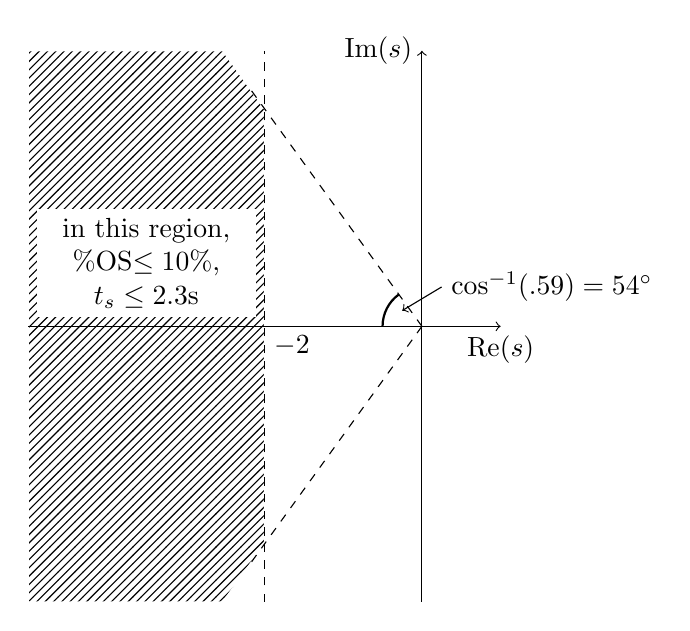
\begin{tikzpicture}

\draw[pattern=north east lines,draw=white] (-5,-3.5) -- (-2.53,-3.5) -- (-2,-2.76) -- (-2,2.76) -- (-2.53,3.5) -- (-5,3.5) -- cycle;
\draw[dashed] (0,0)  -- (-2.17,3);
\draw[dashed] (0,0) -- (-2.17,-3);
\draw[dashed] (-2,-3.5) -- (-2,3.5);
\draw (-2,0) node[below right] {$-2$};
\draw[thick] (-.5,0) arc (180:126:.5);
\draw[->] (-5,0) -- (1,0) node[below] {$\mbox{Re}(s)$};
\draw[->] (0,-3.5) -- (0,3.5) node[left] {$\mbox{Im}(s)$};
\draw (.25,.5) node[right] (cos) {$\cos^{-1}(.59)=54^{\circ}$};
\draw[->] (cos.180) -- ++(-.5,-.3);
\draw (-3.5,.8) node[fill=white] {\begin{minipage}{1.0in}\begin{center}in this region, \%OS$\leq 10$\%, $t_{s}\leq2.3$s\end{center}\end{minipage}};
\end{tikzpicture}
\end{center}

Steps 3-6 will be illustrated at points in Sections \ref{sec:csdesigner}-\ref{sec:verifying}.

\subsection{Using control system designer (sisotool)}\label{sec:csdesigner}
The Mathworks has a tool called the ``Control System Designer'' that was formerly known as ``sisotool'' (which explains the origin of the command that calls the tool). This tool is very helpful for control design, including via root locus.
%To assist us with the design, we will use a control design tool in \textsc{Matlab} called sisotool. 

First, let's enter the system transfer function in the \textsc{Matlab} Command Window \\


\begin{alltt}
>> s=tf([1 0],1)
>> sys=1/((s+10)*(s\^{}2+3*s+2))
\end{alltt}

\noindent The design tool is initialized by typing \texttt{sisotool} at the command prompt.\\

\noindent\texttt{>> sisotool}\\

The following window -- or something similar, depending on your version of \textsc{Matlab} -- will open.

\begin{frame}
\begin{center}
\includegraphics[width=6in]{figures/csdesigner1}
\end{center}
\end{frame}

Click on "Edit Architecture". It opens up the following window

\begin{frame}
\begin{center}
\includegraphics[height=2.8in]{figures/csdesigner3}
\end{center}
\end{frame}

This shows the architecture of the control system that we will be working with. The yellow blocks represent fixed blocks (system and sensor dynamics) that can be set, and the green and red blocks are feedforward and feedback control blocks that can be designed. 

Enter \texttt{sys} in the \textsf{Value} column for the \textsf{G} block to set this block to the transfer function you entered at the command line. Click \textsf{OK}, and the main designer window will change. Note that in the upper right corner, the root locus when the open loop system is \texttt{sys} is shown. 

\begin{frame}
\begin{center}
\includegraphics[height=2.8in]{figures/csdesigner4}
\end{center}
\end{frame}

This is a root locus plot for the current loop gain $H(s)G(s)C(s) = \frac{1}{(s+10)(s^{2}+3s+2)}$. The blue lines are the three loci that make up the root locus plot (all of which are the same color in this tool), and the blue 'x's indicate the open loop poles. Since currently $C(s)=1$, the closed loop poles are at the locations associated with $K_{d}=1$, and no $s+a$ term. These closed-loop poles are indicated by the little pink squares. 

Now, we will put our closed loop pole performance region on this plot. Right click on the root locus plot, and select ``Design Requirements -> New''. Note that settling time is one of the choices. Annoyingly, in this case Matlab defaults to 2\% settling time, so we need to convert our 1\% specification accordingly. Since the 2\% settling time specification is $3.9/\omega_{n}$, while the 1\% settling time specification is $4.6/\omega_{n}$, we should enter
\[
t^{scaled}_{s} = t_{s}\times \frac{3.9}{4.6}. 
\]
So, choose settling time from the menu, and enter $2.3\times \frac{3.9}{4.6}=1.95 $ seconds. Right click and select ``Design Requirements -> New'' again to enter a percent overshoot specification of less than 10\%. The SISO Design window will now look like the following


\begin{frame}
\begin{center}
\includegraphics[height=2.8in]{figures/csdesigner5}
\end{center}
\end{frame}

The white portion is the acceptable region, while the yellow shading indicates that closed loop poles in this region are not acceptable. Note that the root locus on the right does not enter the white region. These would be the dominant poles for the closed loop system, so proportional control alone will not be sufficient to meet the specifications. To implement PD control, we will want to use a controller of the form
\[
C(s) = K(s+a).
\]
\vspace{10pt}
\noindent \textbf{Step 3:} We will start by adding the term $(s+a)$, which corresponds to a zero. On the upper left of the SISO Design window, there is a red circle. If you hover the cursor over it, a help box will say ``add real zero''. Click on the red circle, and then click on the location s=-14+j0 on the root locus plot. The root locus plot will now have changed to the following:

\begin{frame}
\begin{center}
\includegraphics[height=2.8in]{figures/csdesigner6}
\end{center}
\end{frame}

We can check that the control $C(s)$ has been changed by going back to the main window, and click on \textsf{C} in the Data Browser window. Below, the preview window gives the current value for $C(s)$.

\begin{frame}
\begin{center}
\includegraphics[height=1.5in]{figures/csdesigner7_1}\includegraphics[height=1.5in]{figures/csdesigner7_2}
\end{center}
\end{frame}

Note that it says that $C(s) = 0.071353(s+14.1)$. You can verify that this has a zero at $-14.1$, which is apparently where we actually clicked on the graph. 

\vspace{10pt}
\noindent \textbf{Step 4:} Now go back to the SISO Design window. Hover the cursor over the zero that we inserted. You should see the cursor change to a hand symbol. Now click to ``grab'' the zero, and drag the cursor slowly to the right. Note that the root locus plot is updated to reflect the change in this zero location. Keep moving to the right until the root locus for the dominant poles just enters the acceptable region, and let go. The result should look something like the following

\begin{frame}
\begin{center}
\includegraphics[height=2.8in]{figures/csdesigner8}
\end{center}
\end{frame}

Now the root locus will go through the acceptable region, but we still need to choose a gain to get us there. Remember that as the gain increases the closed loop poles move along the root loci to either an open loop zero or infinity. Using the cursor, you can grab one of the pink squares and move it. Notice that this moves all the pink squares in tandem. Move the closed loop poles until the dominant poles lie inside the acceptable pole region. The result should look like the following:

\begin{frame}
\begin{center}
\includegraphics[height=2.8in]{figures/csdesigner9}
\end{center}
\end{frame}

To see what the resulting control $C(s)$ is, go back to the preview.

\begin{frame}
\begin{center}
\includegraphics[height=1.5in]{figures/csdesigner10}
\end{center}
\end{frame}

The designed controller is thus
\[
C(s) = 15.657(s+5.074) = 79.44 + 15.657s 
\]
\vspace{10pt}
\noindent \textbf{Step 5:} In other words, this controller corresponds to a proportional gain of $K_{p}=79.44$ and a derivative gain of $K_{d}=15.66$. 


\subsection{Verifying the Design} \label{sec:verifying}
\noindent \textbf{Step 6:} We can verify if this meets the control specification by plotting the closed loop step response at the \textsc{Matlab} command line or using Simulink. A useful command in \textsc{Matlab} is \texttt{feedback}, which will simplify a feedback loop for us. If we type \texttt{help feedback} at the \textsc{Matlab} command line, we get the following information:

\begin{alltt}
feedback  Feedback connection of two input/output systems. 

M = feedback(M1,M2) computes a closed-loop model M for the feedback loop: 

u --->O---->[ M1 ]----+---> y
|               |           y = M * u
+-----[ M2 ]<---+
...
\end{alltt}
(the help file also continues after this with more information) Note that the two arguments of the \texttt{feedback} command are the transfer functions in the forward and reverse path, respectively.

To check our design, we need to enter in the transfer functions for our implementation feedback loop, which is repeated here with loops separated for emphasis.
\begin{frame}
\begin{center}
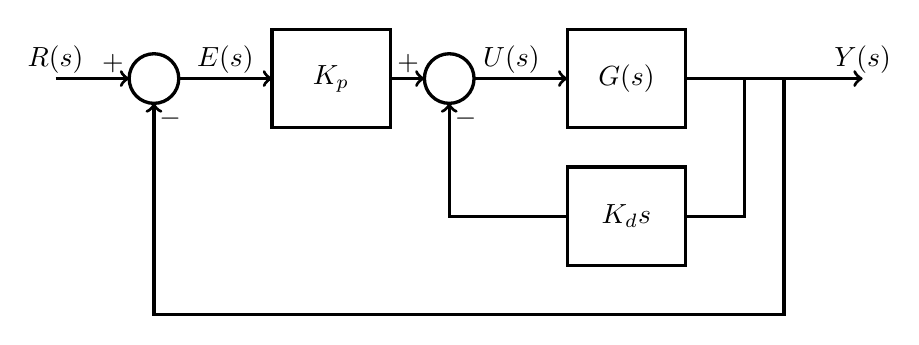
\begin{tikzpicture}[scale=1,inner sep=0pt,outer sep=0pt,very thick,
sysblock/.style={draw,rectangle,inner sep=2pt,minimum width=1.5cm,minimum height=1.25cm,very thick}]

\draw (1.25,0) node[draw,circle] (sum1) {$\rule{0pt}{18pt}$};
\draw (3.5,0) node[sysblock] (Kp) {$K_{p}$};
\draw (5,0) node[draw,circle] (sum3) {$\rule{0pt}{18pt}$};
\draw (7.25,0) node[sysblock] (G) {$G(s)$};
\draw (7.25,-1.75) node[sysblock] (Kd) {$K_{d}s$};

\draw[->] (0,0) node[above=2pt] {$R(s)$} -- (sum1.180) node[above left=2pt] {$+$};
\draw[->] (sum1.0) --  node[above=2pt,pos=.5] {$E(s)$} (Kp);
\draw[->] (Kp) -- (sum3.180) node[above left=2pt] {$+$};
\draw[->] (sum3.0) -- node[above=2pt,pos=.4] {$U(s)$}  (G);
\draw[->] (G) -- ++(3,0) node[above=2pt] {$Y(s)$};
\draw[->] (G) ++(1.5,0) |- (Kd) -| (sum3.-90) node[below right=2pt] {$-$};
\draw[->] (G) ++(2,0) -- ++(0,-3) -| (sum1.-90) node[below right=2pt] {$-$};
\end{tikzpicture}

\end{center}
\end{frame}

The following commands will find the closed loop transfer function $T(s) = \frac{Y(s)}{R(s)}$ for our design. Note that we assume that \texttt{s} has already been defined as the Laplace variable $s$ and \texttt{G} has already been entered as done earlier in this section. We are also using %the gains from Section \ref{sec:sisotool} which are close to but slightly different from the 
slightly different gains from Section \ref{sec:csdesigner}

\begin{alltt}
>>  Kd = 16.01
>>  Kp = 84.25
>>  Inner = feedback(G,Kd*s) \% find transfer function for inner loop
>>  T = feedback(Inner*Kp,1) \% find closed loop transfer function 
\end{alltt}

We can now find the closed loop step response
\begin{frame}
\begin{alltt}
>> step(T)
\end{alltt}
\begin{center}
\includegraphics[width=4in]{figures/PDdesigncheck}
\end{center}
\end{frame}
and verify the step response specifications.
\begin{alltt}
stepinfo(T,{\T}SettlingTimeThreshold\T,.01)

ans = 

RiseTime: 0.586472325105971
SettlingTime: 1.954623565535615
SettlingMin: 0.728640511065229
SettlingMax: 0.879716710297188
Overshoot: 8.855153766744039
Undershoot: 0
Peak: 0.879716710297188
PeakTime: 1.278713133961483
\end{alltt}

%\section{Application Example}
%%\textit{Related to general concepts in the lecture}
%
%\noindent Consider again the wind turbine system in feedback with controller \(C(s)\) in Figure \ref{fig:turbineSys}, where
%\begin{equation*}
%	G_2(s) = \frac{-21.201(s^2+0.04283s+6.509)}{(s+0.2867)(s^2+0.2996s+6.477)}
%\end{equation*}
%
%\begin{figure}
%\begin{center}
%	\includegraphics[width = 4in]{figures/FeedbackLoop.png}\\
%	\caption{Wind turbine plant with feedback control loop and disturbance input.}
%	\label{fig:turbineSys}
%\end{center}
%\end{figure}
%
%Previously (Lecture \RootLocusINumber), we talked about the two cases where the controller is P or PI. Now, let's consider a PD controller:
%\begin{equation*}
%	C(s) = K_p + K_Ds = K_D(s+\frac{K_p}{K_D}),
%\end{equation*}
%which leaves us with two design variables: a zero at \(-K_P/K_D\) and a gain \(K_D\). Plotting the root locus of $-G_2(s)$ in sisotool (Figure \ref{fig:rootLocusPD}) results in the same root locus we've seen before. Recall also that we have some oscillatory behavior in our step response from \(\omega_{ref}\) to \(\omega\), as shown in Figure \ref{fig:stepResponse}. This oscillatory behavior is caused by the lightly damped complex poles located near the imaginary axis.
%
%\begin{figure}
%\begin{center}
%	\includegraphics[width = 4in]{figures/RootLocusEditor.png}\\
%	\caption{Root locus of \(-G_2(s)\). Closed loop poles (pink squares) shown correspond to \(K_D = 0.058\).}
%	\label{fig:rootLocusPD}
%\end{center}
%\end{figure}
%
%\begin{figure}
%\begin{center}
%	\includegraphics[width = 4in]{figures/StepResponse.png}\\
%	\caption{Closed-loop step response when \(K_D = 0.058\). ``Amplitude'' is the rotational frequency \(\omega\) of the wind turbine, and the title ``Step Response'' means that the reference input \(r(t)\) is a unit step function.}
%	\label{fig:stepResponse}
%\end{center}
%\end{figure}
%
%\noindent \textbf{Question:} Thinking of the mechanical structure of the wind turbine, what do you think might be problematic about the step response in Figure \ref{fig:stepResponse}?
%
%\noindent \textbf{Answer:} Lots of oscillations in speed could be damaging to the drive train\\
%
%\noindent \textbf{Question:} Given the root locus shown in Figure \ref{fig:rootLocusPD}, will including another real zero in the controller change the damping significantly?
%
%\noindent \textbf{Answer:} No, because there is a set of complex zeros very near to the set of complex poles, and the loci (representing the possible closed-loop pole locations) connect these complex open loop poles to the complex open loop zeros. Any real zero we add by using PD control design will change the locus on the real axis only, and won't substantially change these complex, dominant closed-loop poles. For example, setting \(K_P/K_D = 1\) and keeping \(K_D = 0.058\) results in the root locus and step response plots shown below.
%
%\begin{center}
%	\includegraphics[width = 3in]{figures/RootLocusEditor2.png}
%	\includegraphics[width = 3in]{figures/StepResponse2.png}
%\end{center}
%

\section{Lecture Highlights}
The primary takeaways from this article include
\begin{enumerate}
\setlength{\itemsep}{5pt}
\setlength{\parskip}{0pt}
\setlength{\parsep}{0pt}
\item Root locus plots can be used to design PID controllers by showing whether, and for what values of a gain $K$, the dominant closed loop poles lie within the allowable region. The allowable region is determined from the rise time, settling time, and percent overshoot specifications for the closed-loop step response.
\item Matlab's \texttt{sisotool} is handy for root-locus based design because it allows easy manipulation of the controller gains and the location(s) of any controller poles and zeros. It can show the closed loop step response plot in real time to enable rapid tuning of these gains until specifications are met.
\end{enumerate}


\section{Quiz Yourself}

\subsection{Questions}

\begin{enumerate}
\setlength{\itemsep}{5pt}
\setlength{\parskip}{0pt}
\setlength{\parsep}{0pt}
\item An electro-magnet can be used to balance a ball made out of a ferromagnetic material. However, for a fixed current, the force on the object becomes stronger when the ball moves closer, and weaker when the ball moves farther away, and thus the system is unstable in open loop.
\begin{center}
\input{quizfigures/maglev.tex}
\end{center}
The transfer function for a magnetic levitation system has the form
\[
\frac{Y(s)}{I_{in}(s)} = \frac{K_{0}}{(s^{2} - a^{2})(s+\tau)}
\]
You wish to use a PD control system to stabilize the mag-lev system and achieve a $1 \%$ settling time less than 1.3 seconds and \%OS less than $10\%$. 
\begin{center}
\input{quizfigures/maglevcontrol.tex}
\end{center}
Suppose the parameters are $K_{0}=10$, $a=1$ and $\tau=10$.
\begin{enumerate}
\item Sketch the root locus for $K_{d}=0$, and indicate the allowable closed loop pole regions.
\item Using the technique from class, choose $K_{d}$ and $K_{p}$ to place the closed loop poles on or inside the allowable region.
\item Find the closed loop transfer function $Y(s)/R(s)$. Using \texttt{Matlab} find the step response to verify that your design specifications have been met. 
\end{enumerate}
\end{enumerate}

\subsection{Solutions}
\begin{enumerate}
\setlength{\itemsep}{5pt}
\setlength{\parskip}{0pt}
\setlength{\parsep}{0pt}
\item \rule{0pt}{12pt}\\
\begin{enumerate}
\item
\begin{center}
\includegraphics[width=4in]{quizfigures/1asoln}\\
\includegraphics[width=4in]{quizfigures/1bsoln}
\end{center}
\item Using SISOtool, we enter in the constraints and choose a zero to move the root locus inside the constraint region
\begin{center}
\includegraphics[height=2.8in]{quizfigures/1csoln}
\end{center}
The resulting controller is shown in the Control and Estimation Tools Manager
\begin{center}
\includegraphics[height=2.8in]{quizfigures/1dsoln}
\end{center}
\item \rule{0pt}{0pt}
\begin{center}
\includegraphics[width=4in]{quizfigures/1esoln}\\
\includegraphics[width=4in]{quizfigures/1fsoln}
\end{center}

\end{enumerate}
\end{enumerate}



\end{document}


